\section{The Colony Network}\label{sec:colonynetwork}

The Colony Network is a collection of contracts on the Ethereum blockchain. At the core of the network is the \code{ColonyNetwork} contract. This contract is primarily responsible for managing the reputation mining process (see Section \ref{sec:reputationmining}), but also for general management of the network: deploying new colonies, setting the fees associated with using the network, and releasing new versions of the \code{Colony} contracts. These actions will be mediated by a special colony, the \rc.

\subsection{Revenue model}\label{sec:networkrevenue}

The Colony Network must be able to sustain itself. In particular, the \rc\ (which controls the Colony Network) maintains the contracts that underpin the network and develops new functionality for the network --- development of which needs to be paid for. Long term, the development and maintenance of the network (including the reputation system) needs to be financed by the network itself.

\subsubsection{The network fee}\label{sec:networkfee}

We propose a fee levied on expenditure and reward payouts. When a user claims a payout, some small fraction will be paid to the network. The fees are sent to either the \rc\ (if the payment was in Ether or another whitelisted `currency' token) or the Colony Network contract (if it is any other ERC20-compatible token). A cartoon showing the revenue split is show in Figure \ref{fig:revenueSplit}.

\begin{figure}[htp]
\centering
 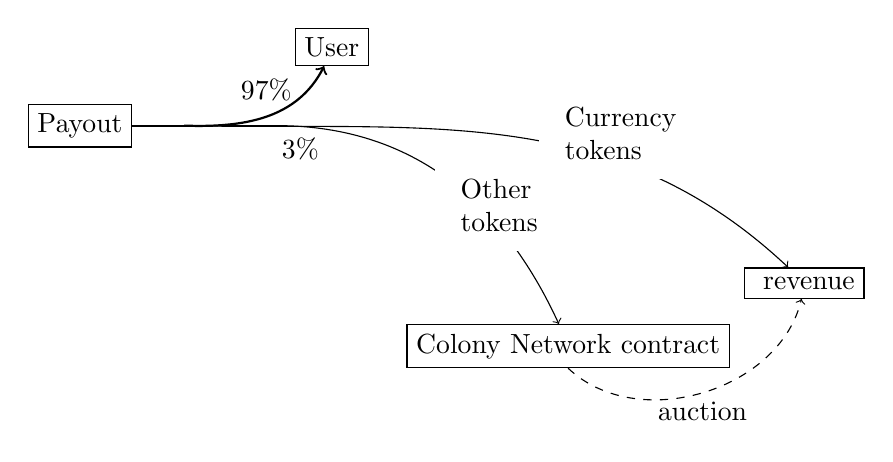
\begin{tikzpicture}
  \node at (-4,0) (dummy) {};
  \node[draw] at (-5.2,0) (bountybox) {Payout};
  \node at (-2.8,0) (bounty) {}
   (bountybox.east) edge[-, thick] (dummy.east)
   (dummy.east) edge[-] (bounty.east);
   \node at (-2.4,-0.3) {{3\%}};
  \node[draw] at (-2,1) (user) {User};
  \node[draw] at (1,-2.8) (cnc) {Colony Network contract};
  \node[draw] at (4,-2) (root) {\rc\ revenue}
    (dummy.east) edge[->, bend right=40,out=-25,thick] node[above=2pt] {97{\%}} (user)
    (dummy.east) edge[->, bend left=30,out=12] node[fill=white,right=10pt] {\begin{tabular}{l} Currency \\ tokens\end{tabular}} (root)
    (bounty.east) edge[->, bend left=30,out=35] node[fill=white, below right=-5pt] {\begin{tabular}{l} Other \\ tokens\end{tabular}} (cnc)
    (cnc.south) edge[->, bend right=60, dashed] node[below] {auction} (root)
    ;
 \end{tikzpicture}
 \caption{Summary of the revenue split upon payout for a task.}
 \label{fig:revenueSplit}

\end{figure}

This idea of a fee is a little unusual for such a decentralised system. One of the appeals of decentralised systems on Ethereum is that other than gas costs, they do not seek rent and are free to use. However, the network fee is key to ensuring the game theoretic security of the Colony Network's reputation mining and governance processes, by providing underlying value to the CLNY held by Meta Colony members. Importantly, this fee is not payable to any centrally controlled entity, but rather to the Meta Colony. As anybody may contribute to the Meta Colony, anyone may claim a share of these fees proportional to their contribution. We believe that the benefit of being part of a secure, well maintained network will be appealing enough that a small fee to pay for its existence will be acceptable.

The presence of this fee means we have to make some considerations which would otherwise be irrelevant. Primarily, we will need to make `piggyback' contracts as hard as possible to make that might e.g. be used to pay out an expenditure payout when a expenditure was finalized, but without sending the fee.

\subsubsection{The token auction}

As the network fee may be denominated in any ERC20 token, there is a need for a mechanism to liquidate arbitrary bundles of tokens: the token auction. The tokens collected are auctioned off by the Colony Network Contract, with the auctions denominated in \rcts, the proceeds of which are burnt. These auctions --- one for each type of token collected --- occur on a regular basis of once a month.

We believe such a mechanism will be beneficial for the \rcths\ (whose tokens gain value by having an explicit use beyond reputation mining) and the \rc\ itself (by reducing the supply of \rcts\ and thus making any future minting more valuable). It also provides an immediate mechanism of price discovery for a colony's internal tokens, which are unlikely to be traded on third-party exchanges until much later in the lifetime of the colony. By auctioning off the collected tokens, we also prevent the \rc\ collecting a large number of different tokens that it has to manage, which would prove cumbersome and annoying.

\subsection{The \rc\ and CLNY}\label{sec:clny}

The \rc\ is a special colony which governs the Colony Network. Tokens in the \rc\ are known as CLNY and will be initially generated during the Colony Network distribution period.\footnote{The mechanism of this distribution are yet to be defined.}

\subsubsection{Role of CLNY holders and the \rc}

CLNY holders have two primary roles. The first is to participate in the reputation mining process, described in Section \ref{sec:reputationmining}. The second is management of the Colony Network itself. There will be permissioned functions on the Network Contract to allow fundamental parameters of the network to be set, which can only be called by the \rc. For these permissioned functions to be called by the \rc, a vote open to all CLNY and reputation holders must be conducted.

Management of the Colony Network also includes making updates to Colony contracts available to colonies. CLNY holders are not necessarily responsible for the development of these updates, but are required to vote to deploy them. They are therefore responsible for at least ensuring due diligence is done, either by themselves or by service providers, to avoid introducing security weaknesses or other undesirable behaviour. In return for the responsibility of the development and maintenance of the Colony Network, the \rc\ is the beneficiary of the network fee (see Section \ref{sec:networkrevenue}).

Reputation in the \rc\ can be acquired by earning CLNY tokens by via expenditure payouts just as in any other colony (see Section \ref{sec:earning-losing-rep}). Reputation in the \rc\ can also be earned by participating in the reputation mining process (see Section \ref{subsec:mining-costs-and-rewards}), which is unique to the \rc.

\subsubsection{Handing off decision-making power to the \rc}\label{subsec:ceding-control-to-rc}

\rct\ holders are responsible for reputation mining from the start, but decisions about the underlying properties of the network will initially be made by a multisignature contract controlled by the Colony team. As the network develops and is proved to be effective, control over these decisions will cede to the \rc.

\subsubsection*{Stage 1: Colony team multisig in control}
 Initially, the Network Contract's functions will be \textbf{root}-permissioned to only allow transactions from the multisig contract under the control of the Colony team to change these properties of the network.

\subsubsection*{Stage 2: Colony team multisig approval required}
At a later date, an extension contract will be set up and given the \textbf{root} permission. This contract will allow the \rc\ (as a whole, via the governance mechanisms provided to all colonies) to propose changes to be made to the Colony Network Contract. The intermediate contract will have functionality such that all changes will have to be explicitly allowed by the account under the control of the Colony team. In other words, the \rc\ will be able to propose changes, but the team must sign them off.

\subsubsection*{Stage 3: Colony team multisig retains veto}
The next stage will be a second extension contract operating similarly to the first, but after a timeout --- with no interaction from the Colony team's account --- the change will be able to be forwarded to the Colony Network Contract by anyone. The Colony team's role will be to block changes if necessary. Thus at this stage the \rc\ will be able to make changes autonomously, but the Colony team retains a veto.  The proposal to move to this contract will have to come from the \rc\ itself.

\subsubsection*{Stage 4: \rc\ fully controls the network}
Finally, the specialized extension contract will be removed and replaced with a generic voting extension (see Section \ref{sec:objections-and-disputes}), and the \rc\ will have direct control over the Colony Network Contract with no privileged control available to the Colony team other than that provided by any CLNY and reputation held.
